\section{Analisi dei Dati}

Per fare l'operazione di analisi dei dati si è utilizzato Google Colab \cite{googlecolab}, un ambiente di sviluppo gratuito basato su cloud che offre l'accesso a potenti risorse di calcolo tramite browser, consentendo agli utenti di scrivere, eseguire e condividere codice Python.

Questa operazione di analisi si è concentrata sulle prestazioni dell'algoritmo e sui thread che lavorano all'interno di esso.

\subsection{Prestazioni algoritmo}
La seguente documentazione è presente in formato originale con il codice Python utilizzato, come notebook di Google Colab al seguente link:

{\footnotesize \href{https://colab.research.google.com/drive/1PZyxKQf85-XFKB7PsUqYRUQSwh0I-cuO?usp=sharing}{https://colab.research.google.com/drive/1PZyxKQf85-XFKB7PsUqYRUQSwh0I-cuO?usp=sharing}}

\subsubsection{Analisi prestazioni algoritmo}
Il seguente notebook viene utilizzato per fare un'analisi dei dati per verificare il requisito non funzionale della performance:

L’algoritmo di priorità impiegato dalla cucina per la selezione degli ordini deve fornire risultati in un tempo utile.

\subsubsection{Analisi file di report}
Viene caricato e visualizzato il file di report in formato csv che da in output l'algoritmo:

\begin{figure}[H]
	\centering
	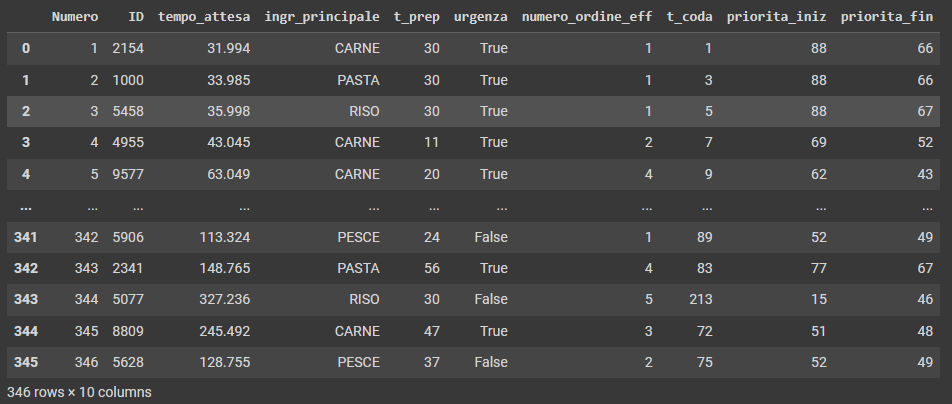
\includegraphics[scale=0.6]{iterazione3/images/datasetcsv.png}
	\caption{File csv di report\label{fig:report-csv}}
\end{figure}

\subsubsection{Analisi Tempo di attesa in base al numero degli ordini}
Come primo passo viene analizzato come il tempo di attesa varia con l'avanzare del numero di ordini.

Viene utilizzato un grafico a linea per mostrare (in arancione) il tempo di attesa per numero di ordine e (in blu) i valori filtrati con un filtro a media mobile con finestra = 10 valori

\begin{figure}[H]
	\centering
	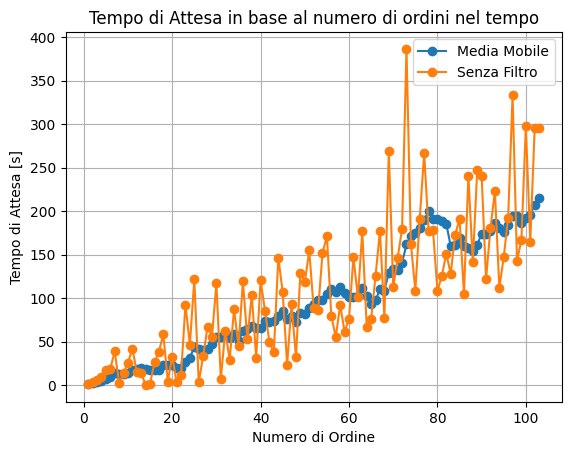
\includegraphics[scale=0.6]{iterazione3/images/t_attesa_numero_ordini.png}
	\caption{Analisi Tempo di attesa in base al numero degli ordini\label{fig:lineplot}}
\end{figure}

Si può notare come con l'aumentare del numero di ordini il tempo di attesa continui a salire quasi in maniera costante, questo è dovuto al fatto che la domanda nel periodo di osservazione è costante e superiore alla capacità della cucina, così gli ordini si accumulano in coda.

\subsubsection{Analisi distribuzione del tempo di attesa di preparazione degli ordini}
In questa sezione viene analizzato il tempo di attesa di preparazione degli ordini, ossia il tempo che passa da quando un ordine viene effettuato a quando viene preso in carico dal cuoco, non viene considerato quindi il tempo di preparazione poiché caratteristico del singolo ordine

Viene utilizzato un istogramma con il quale si mostra la frequenza con la quale i vari ordini presentano un certo slot di tempo di attesa, 
vengono inoltre calcolate e mostrate: media, deviazione standard, mediana, 25° e 75° percentili per una maggiore comprensione.

In un ulteriore istogramma poi si raggruppano queste frequenze in base alla priorità, con valori di Alta, Media e Bassa priorità per capire come l'assegnazione della priorità da parte dell'algoritmo influenza il tempo di attesa di preparazione.\\
$Media tempo di attesa = 128.982s$\\
$Deviazione standard tempo di attesa = 79.019s$\\
$Mediana standard tempo di attesa = 119.218s$\\
$25° percentile tempo di attesa = 75.894s$\\
$75° percentile tempo di attesa = 171.767s$
\begin{figure}[H]
	\centering
	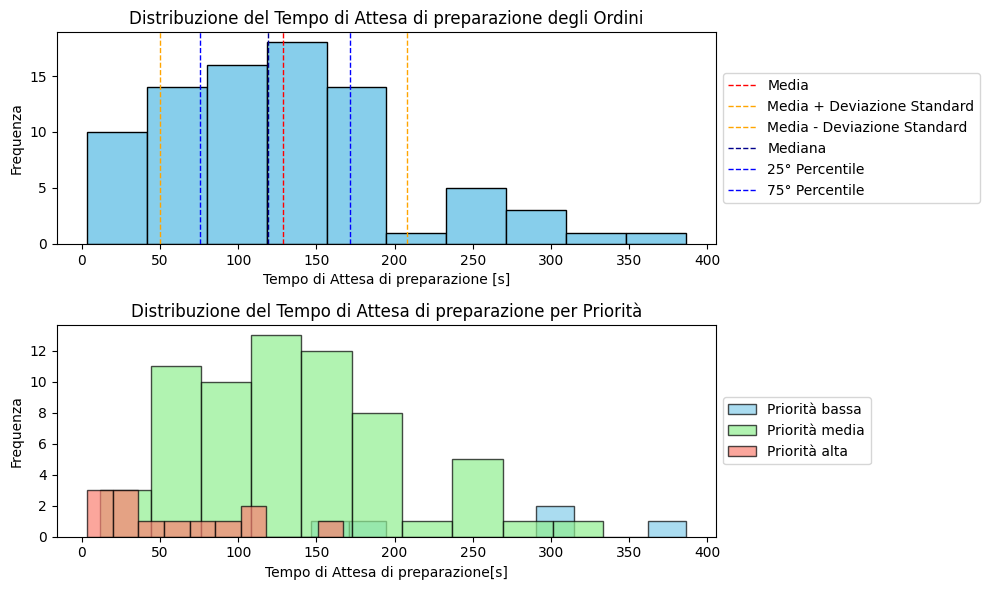
\includegraphics[scale=0.6]{iterazione3/images/distr_t_attesa_prep.png}
	\caption{Distribuzione del Tempo di Attesa di preparazione degli Ordini\label{fig:distr_t_attesa_prep}}
\end{figure}
Dal primo istogramma è possibile notare che:
\begin{itemize}
	\item la media è di poco superiore alla mediana, ciò può fare pensare che la distribuzione sia approssimativamente simmetrica;
	\item significativa deviazione standard, ciò indica che c'è una variabilità nei tempi di attesa;
	\item presenza di outlier: dati molto al di fuori dell'intervallo tra il 25° e il 75° percentile, potrebbero essere considerati outlier o dati anomali.
\end{itemize}
Dal secondo istogramma è invece possibile notare come tendenzialmente le priorità siano rispettate, con ordini che hanno una priorità maggiore che presentano un tempo di attesa di preparazione minore.

\subsubsection{Analisi distribuzione del tempo di attesa in coda degli ordini}
In questa sezione viene analizzato il tempo di attesa in coda degli ordini, ossia il tempo che passa da quando un ordine viene effettuato a quando viene esce dalla coda per andare in cucina, non viene considerato quindi il tempo di preparazione e il tempo di attesa in cucina.

Viene utilizzato un istogramma con il quale si mostra la frequenza con la quale i vari ordini presentano un certo slot di tempo di attesa, vengono inoltre calcolate e mostrate: media, deviazione standard, mediana, 25° e 75° percentili per una maggiore comprensione.

In un ulteriore istogramma poi si raggruppano queste frequenze in base alla priorità, con valori di Alta, Media e Bassa priorità per capire come l'assegnazione della priorità da parte dell'algoritmo influenza il tempo di attesa di preparazione.\\
$Media tempo di attesa = 73.084s$\\
$Deviazione standard tempo di attesa = 67.694s$\\
$Mediana standard tempo di attesa = 61.000s$\\
$25° percentile tempo di attesa = 10.000s$\\
$75° percentile tempo di attesa = 113.500s$
\begin{figure}[H]
	\centering
	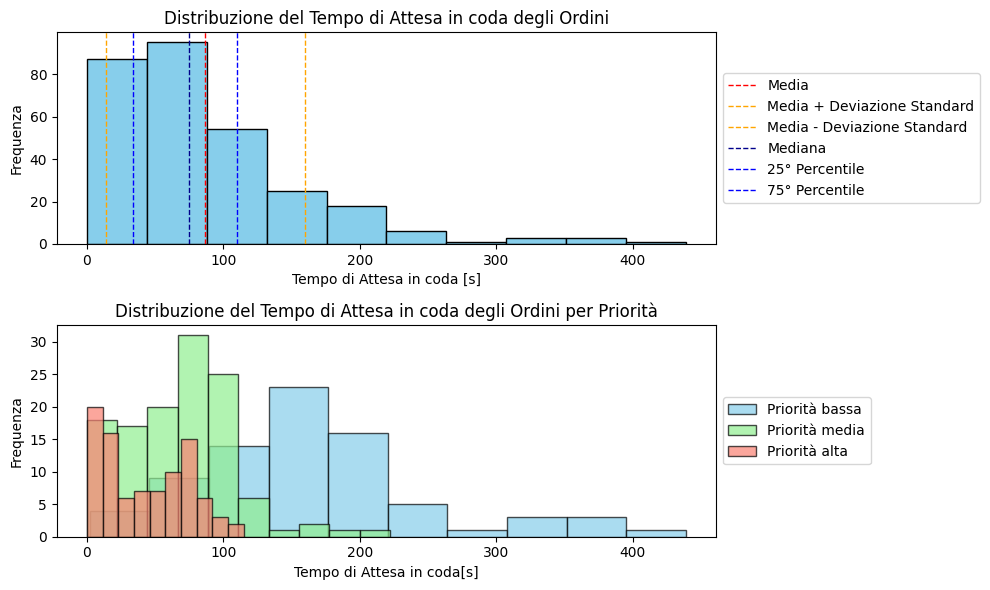
\includegraphics[scale=0.6]{iterazione3/images/distr_t_attesa_coda.png}
	\caption{Distribuzione del Tempo di Attesa in coda degli Ordini\label{fig:distr_t_attesa_coda}}
\end{figure}
Questi grafici sono simili ai grafici calcolati precedentemente per il tempo di attesa di preparazione, per cui si possono tirare le stesse conclusioni, si può inoltre notare che ci sono molti ordini a priorità media e alta che presentano tempi di attesa in coda nulli o poco superiori allo zero, possiamo ipotizzare che l'alta frequenza di ordini con basso tempo di attesa in coda sia data dagli ordini effettuati inizialmente questo perché è possibile che al momento della loro ordinazione trovino il buffer vuoto o comunque poco carico e vengano quindi subito spediti alla cucina.
\begin{figure}[H]
	\centering
	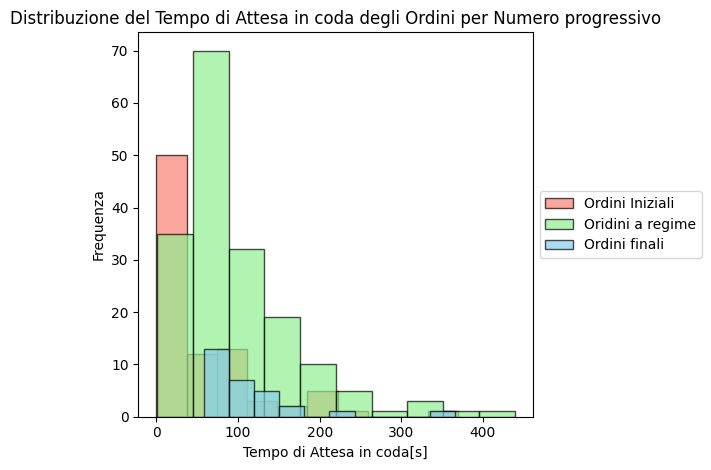
\includegraphics[scale=0.6]{iterazione3/images/distr_t_attesa_coda_nrordine.png}
	\caption{Distribuzione del Tempo di Attesa in coda degli Ordini per Numero progressivo\label{fig:distr_t_attesa_coda_nrordine}}
\end{figure}
Viene infatti confermata l'ipotesi del passo precedente e cioè che gli ordini che presentano tempi di attesa in coda nulli o poco superiori allo zero siano dati principalmente da ordini effettuati nelle fasi iniziali.

\subsubsection{Analisi dei parametri in base al tempo totale in attesa}
In questo passo viene analizzato come i 5 parametri su cui si basa la priorità influiscano sul tempo di attesa di un ordine nel sistema, cioè da quando viene effettuato a quando viene completato. I parametri in considerazione sono:
\begin{itemize}
	\item ingrediente principale, indica la postazione della cucina riservata a quel particolare ordine;
	\item tempo di preparazione, rappresenta la durata stimata necessaria per preparare un determinato ordine;
	\item urgenza del cliente, consente ai clienti di specificare la tempestività con cui desiderano ricevere il proprio ordine;
	\item numero ordine effettuato, specifica il numero dell’ordine del cliente in ordine temporale (posizione relativa di un ordine all’interno della sequenza di ordini effettuati da egli stesso);
	\item tempo in attesa in coda, rappresenta il periodo di tempo trascorso da quando un ordine è stato effettuato fino al momento in cui viene elaborato.
\end{itemize}
\begin{figure}[H]
	\centering
	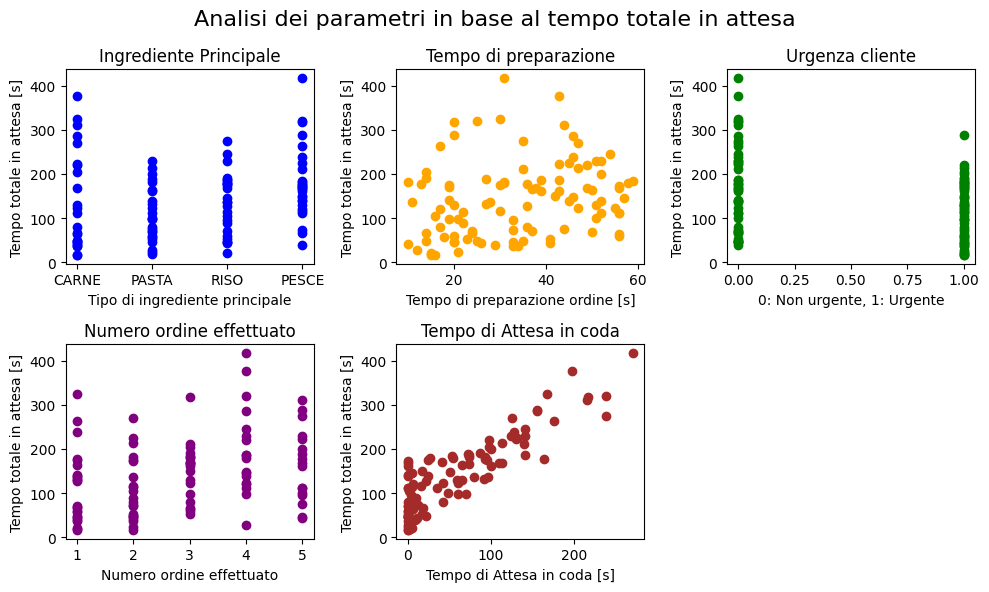
\includegraphics[scale=0.6]{iterazione3/images/analisi_parametri.png}
	\caption{Analisi dei parametri in base al tempo totale in attesa\label{fig:analisi_parametri}}
\end{figure}

\subsection{Analisi dei thread}

\clearpage